\documentclass[11pt,a4paper]{article}

\usepackage[a4paper,margin=22mm,headheight=14pt]{geometry}
\usepackage{amsmath,amssymb,mathtools,bm}
\usepackage{booktabs,tabularx,array,longtable,multirow}
\usepackage{microtype}
\usepackage{xcolor}
\usepackage{enumitem}
\usepackage{fancyhdr}
\usepackage{hyperref}
\usepackage{pdflscape}
\usepackage{tikz}
\usetikzlibrary{arrows.meta,positioning,fit,calc,backgrounds,shapes.geometric}

\definecolor{FFIndigo}{HTML}{3F3C8F}
\definecolor{FFBlue}{HTML}{276FBF}
\definecolor{FFTeal}{HTML}{188977}
\definecolor{FFOrange}{HTML}{D36B28}
\definecolor{FFRed}{HTML}{B6424A}
\definecolor{FFInk}{HTML}{202632}
\definecolor{FFGray}{HTML}{657184}
\definecolor{FFPale}{HTML}{F1F4F8}
\definecolor{FFGreenPale}{HTML}{E8F4F0}
\definecolor{FFOrangePale}{HTML}{FAEFE7}
\definecolor{FFBluePale}{HTML}{EAF1FA}

\hypersetup{
  colorlinks=true,
  linkcolor=FFIndigo,
  citecolor=FFTeal,
  urlcolor=FFBlue,
  pdftitle={FermiForge: current two-dimensional quasiclassical solver},
  pdfauthor={FermiForge project}
}

\pagestyle{fancy}
\fancyhf{}
\lhead{FermiForge implementation note}
\rhead{20 September 2026}
\cfoot{\thepage}

\setlist[itemize]{leftmargin=1.5em,itemsep=0.25em,topsep=0.35em}
\setlist[enumerate]{leftmargin=1.7em,itemsep=0.25em,topsep=0.35em}
\setlength{\parindent}{0pt}
\setlength{\parskip}{0.55em}
\setlength{\emergencystretch}{2em}

\newcommand{\ii}{\mathrm{i}}
\newcommand{\Tr}{\operatorname{Tr}}
\newcommand{\dd}{\mathrm{d}}
\newcommand{\oneSpin}{\mathbf{1}_{2}}
\newcommand{\oneNambu}{\mathbf{1}_{4}}
\newcommand{\phat}{\hat{\bm p}}
\newcommand{\rhat}{\hat{\bm r}}
\newcommand{\Aop}{A_{\alpha i}}
\newcommand{\Fmap}{\mathcal{F}}
\newcommand{\code}[1]{\texttt{\detokenize{#1}}}
\newcommand{\status}[2]{\textcolor{#1}{\textsf{\bfseries #2}}}

\tikzset{
  >={Latex[length=2.2mm]},
  ffbox/.style={rounded corners=2pt, draw=FFIndigo, thick, fill=FFBluePale,
    align=center, text width=37mm, minimum height=10mm, inner sep=3pt},
  ffgreen/.style={ffbox, draw=FFTeal, fill=FFGreenPale},
  fforange/.style={ffbox, draw=FFOrange, fill=FFOrangePale},
  ffdecision/.style={diamond, aspect=2.2, draw=FFOrange, thick,
    fill=FFOrangePale, align=center, inner sep=1.5pt, text width=28mm},
  ffgroup/.style={rounded corners=4pt, draw=FFGray, dashed, thick,
    inner sep=4mm},
  ffarrow/.style={->, thick, draw=FFInk},
  ffreturn/.style={->, thick, draw=FFOrange}
}

\begin{document}
\hypersetup{pageanchor=false}

\begin{titlepage}
  \centering
  \vspace*{18mm}
  {\Huge\bfseries\color{FFIndigo} FermiForge\par}
  \vspace{4mm}
  {\LARGE Current two-dimensional quasiclassical solver\par}
  \vspace{3mm}
  {\Large Equations, numerical algorithm, and code architecture\par}
  \vspace{16mm}

  \begin{minipage}{0.88\textwidth}
  \color{FFInk}
  This note records the algorithm that is implemented now for a
  translation-invariant two-dimensional cross-section of a spin-triplet
  superfluid.  Its immediate purpose is to make the normal-core, A-phase-core,
  and double-core vortex development auditable.  It also identifies the
  interfaces that can later support walls, leads, discontinuous-Galerkin
  discretisation, and portable accelerator execution.
  \end{minipage}

  \vfill
  \begin{tabular}{rl}
    Document status: & living implementation note, revision 0.1\\
    Snapshot date: & 20 September 2026\\
    Repository: & \url{https://github.com/fogelstrom-lab/FermiForge}\\
    Baseline commit: & \code{3d9897e} plus the current development work tree\\
    Primary executable: & \code{fermiforge_double_core_2d}
  \end{tabular}
  \vspace{12mm}

  {\small
  The words \emph{implemented}, \emph{validation}, \emph{experimental}, and
  \emph{planned} are used deliberately.  They distinguish working code from
  the intended architecture and avoid turning a roadmap statement into a
  claim about the present solver.}
\end{titlepage}

\hypersetup{pageanchor=true}
\pagenumbering{roman}

\tableofcontents
\clearpage
\pagenumbering{arabic}

\section{Executive overview}

The implemented calculation is a nonlinear fixed-point problem for the full
complex triplet order-parameter tensor and a three-component, current-related
Fermi-liquid mean field on a two-dimensional Cartesian cross-section.  Every
MPI rank currently holds the complete spatial state.  Active target points are
distributed among ranks; at each target the code integrates stable coherence
functions along all quasiclassical directions and positive Ozaki poles,
reconstructs the spin--Nambu propagator, and forms a new local mean field.  A
global reduction assembles the mapped field, after which rank zero projects
selected zero modes and applies the source-compatible Anderson accelerator.

The central separation of concerns is
\begin{equation}
  \begin{gathered}
  \boxed{\text{spatial field}}
  \longrightarrow
  \boxed{\text{ray sampling}}
  \longrightarrow
  \boxed{\text{Riccati transport}}\\[2mm]
  \boxed{\text{local self-consistency map}}
  \longrightarrow
  \boxed{\text{nonlinear update}} .
  \end{gathered}
\end{equation}
The field grid, the one-dimensional trajectory integration mesh, and the
nonlinear iteration vector are therefore distinct objects.  This is important
both for multiscale accuracy and for a future GPU implementation.

\subsection*{Maturity at this snapshot}

\begin{tabularx}{\textwidth}{>{\raggedright\arraybackslash}p{27mm}X}
\toprule
\status{FFTeal}{Implemented} & Full complex $3\times3$ triplet field; full
$2\times2$ spin coherence and $4\times4$ spin--Nambu propagator; static
nonuniform rectilinear mesh; Q1 interpolation; straight rays; free-vortex
asymptotic continuation; MPI point distribution; source-compatible Anderson
mixing; checkpointing; optional zero-mode projection.\\
\status{FFBlue}{Validated} & Unit and regression tests for mesh sampling,
radial embedding, trajectory transport, propagator reconstruction,
self-consistency integrands, MPI rank agreement, and normal-core radial/2D map
comparison.  Converged radial normal- and A-core fields are references; this
does not by itself certify every modern 2D relaxation as converged.\\
\status{FFOrange}{Experimental} & Free double-core relaxation, angle-dependent
asymptotic state fitting, dependent-halo regeneration, staged domain studies,
zero-mode removal, and held-out exterior ``shadow'' iteration.\\
\status{FFRed}{Planned} & Error-driven block AMR, discontinuous-Galerkin
transport, container walls and reflection, interfaces/leads, dipole-energy
self-consistency, physical observable normalisations, GPU offload, and
distributed spatial fields.\\
\bottomrule
\end{tabularx}

The present implementation is therefore best described as an
\emph{MPI-enabled research prototype designed for later scaling}, not yet as a
production large-cluster or GPU solver.

\section{Provenance and notation}

The implementation deliberately preserves several numerical conventions from
the working radial code in \code{new_src}.  The physical notation is aligned
with the supplied double-core manuscript~\cite{dcvlong}; where a general
quasiclassical convention and the historical source convention could differ,
the code-compatible quantity is named explicitly rather than silently
identified with a more general object.

The spatial coordinates are $\bm r=(x,y)$ and the vortex axis is $z$, with
$\partial_z=0$.  Momentum remains three dimensional,
\begin{equation}
  \phat=(p_x,p_y,p_z)
  =\left(\sqrt{1-p_z^2}\cos\theta_p,
         \sqrt{1-p_z^2}\sin\theta_p,p_z\right),
  \qquad |\phat|=1 .
  \label{eq:momentum}
\end{equation}
Greek indices $\alpha,\beta\in\{x,y,z\}$ label spin components and Roman
indices $i,j\in\{x,y,z\}$ label orbital components.  Repeated component
indices are summed when this is unambiguous.

The code-basis triplet field is
\begin{equation}
  A_{\alpha i}(\bm r)\in\mathbb{C}^{3\times3},
  \qquad
  d_\alpha(\phat,\bm r)=A_{\alpha i}(\bm r)p_i,
  \label{eq:dvector}
\end{equation}
and the gap matrix is
\begin{equation}
  \widehat\Delta(\phat,\bm r)
  =\sum_{\alpha i}A_{\alpha i}(\bm r),
       \ii\sigma_\alpha\sigma_y p_i
  =(\bm d\cdot\bm\sigma)\ii\sigma_y
  =\begin{pmatrix}
     -d_x+\ii d_y & d_z\\ d_z & d_x+\ii d_y
   \end{pmatrix}.
  \label{eq:gapmatrix}
\end{equation}
The stored real vector $\bm v(\bm r)$ is the coefficient used to construct
the diagonal Fermi-liquid shift.  It is called a
\emph{current-related mean field}; it is not yet a mass current in physical
units.  With the caller-supplied feedback scale $a_{\rm FL}$,
\begin{equation}
  \nu(\phat,\bm r)=a_{\rm FL}\,\phat\cdot\bm v(\bm r),
  \qquad
  a_{\rm FL}=\frac{F_1^s}{1+F_1^s/3}
  \quad\text{in the present run configurations}.
  \label{eq:diagonalshift}
\end{equation}
At each mesh node the nonlinear state consequently has
\begin{equation}
  9\text{ complex }A_{\alpha i}+3\text{ real }v_i=21\text{ real unknowns}.
  \label{eq:statecount}
\end{equation}

\section{Quasiclassical transport problem}

In conventional notation, the equilibrium propagator obeys an Eilenberger
transport equation of the form
\begin{equation}
  \ii\hbar\bm v_F\cdot\bm\nabla\check g
  +[\ii\omega_n\check\tau_3-\check\Sigma,\check g]=0,
  \qquad \check g^2=-\oneNambu,
  \label{eq:eilenberger}
\end{equation}
in the dimensionless normalisation used by the compatibility layer.  The
current code does not integrate the matrix equation directly.  It evolves two
stable Riccati/coherence branches from opposite ends of each ray and
reconstructs $\check g$ at the target~\cite{eschrig2000}.

\subsection{Projected ray and Q1 field sampling}

For target $\bm r_0=(x_0,y_0)$ and direction \eqref{eq:momentum}, the projected
trajectory is
\begin{equation}
  \bm r(s)=\bm r_0+s(p_x,p_y),
  \qquad \bm r(0)=\bm r_0 .
  \label{eq:ray}
\end{equation}
The line is clipped to the rectangular storage mesh, the target is inserted
exactly at $s=0$, and every interval is bounded by a separate trajectory step
control.  A direction parallel to the invariant axis has one spatial sample,
but still retains its full momentum in \eqref{eq:dvector}.

On a rectilinear cell $[x_0,x_1]\times[y_0,y_1]$, set
\begin{equation}
  \xi=\frac{x-x_0}{x_1-x_0},\qquad
  \eta=\frac{y-y_0}{y_1-y_0}.
\end{equation}
The interpolation operator is
\begin{align}
  Q_1[f](x,y)={}&(1-\xi)(1-\eta)f_{00}
    +\xi(1-\eta)f_{10}\nonumber\\
    &+(1-\xi)\eta f_{01}+\xi\eta f_{11}.
  \label{eq:q1}
\end{align}
It acts directly on every complex Cartesian component of $A$ and every real
component of $\bm v$; amplitudes and phases are not interpolated separately.
The four point indices and weights form a reusable stencil.  Thus fixed
geometry can later be cached independently of changing field values.

\subsection{Implemented Riccati coefficient equation}

The exact compatibility kernel stores a coherence function as four complex
coefficients $a=(a_0,\bm a)$.  Let
$\alpha=(\alpha_0,\bm\alpha)$ and
$\beta=(\beta_0,\bm\beta)$ be the local pair coefficients,
$\zeta=\ii z_q-\nu$, and $\bm h$ the spin-vector diagonal self-energy.  The
transcribed ordinary differential equation is
\begin{align}
 \frac{\dd a_0}{\dd s}
 &=\ii\left[(a_0^2+\bm a\cdot\bm a)\beta_0
   +2a_0(\zeta+\bm\beta\cdot\bm a)
   +\alpha_0-2\bm h\cdot\bm a\right],
   \label{eq:riccati0}\\
 \frac{\dd a_j}{\dd s}
 &=\ii\left[(a_0^2-\bm a\cdot\bm a)\beta_j
   +2a_j(\zeta+\bm\beta\cdot\bm a+\beta_0a_0)
   +\alpha_j-2h_ja_0\right].
   \label{eq:riccatij}
\end{align}
For the active pure-triplet calculation,
\begin{equation}
  a_0=\alpha_0=\beta_0=0,\qquad \bm h=0,
\end{equation}
so that
\begin{equation}
  \frac{\dd\bm a}{\dd s}
  =\ii\left[\bm\alpha
       +2(\zeta+\bm\beta\cdot\bm a)\bm a
       -(\bm a\cdot\bm a)\bm\beta\right].
  \label{eq:riccati-triplet}
\end{equation}
On the forward branch $(\bm\alpha,\bm\beta)=(\bm d,\bm d^*)$; on the reverse
branch $(\bm\alpha,\bm\beta)=(\bm d^*,\bm d)$.  These statements describe the
implemented legacy-compatible branches.  They do not yet define the most
general equilibrium tilde operation for arbitrary singlet, triplet, exchange,
and interface self-energies.

At an endpoint the source-compatible bulk value uses
\begin{equation}
  \lambda=\ii\sqrt{\bm\alpha\cdot\bm\beta-\zeta^2},
  \qquad
  \bm a=-\frac{\bm\alpha}{\zeta+\lambda},
  \label{eq:bulkcoherence}
\end{equation}
with the Fortran complex square-root branch.  An optional constant endpoint
segment provides explicit relaxation before propagation through the sampled
path.

Each interval is advanced by classical fourth-order Runge--Kutta while the
self-energy coefficients are linearly interpolated to the RK stages.  For
Ozaki pole $z_q$, the interval substep count is
\begin{equation}
  K_q=\max\!\left(K_{\min},1+\operatorname{int}|z_q|\right).
  \label{eq:substeps}
\end{equation}
This reproduces the radial source arithmetic; it is independent of the maximum
spacing used to construct the trajectory samples.

\subsection{Spin--Nambu reconstruction and normalisation}

Let $a^{\rm F}=(a^{\rm F}_0,a^{\rm F}_x,a^{\rm F}_y,a^{\rm F}_z)$ and
$a^{\rm R}=(a^{\rm R}_0,a^{\rm R}_x,a^{\rm R}_y,a^{\rm R}_z)$ denote the
coefficient sets returned by the forward and reverse integrations.  The
forward matrix is
\begin{equation}
  \gamma
  =(a^{\rm F}_0\oneSpin+\bm a^{\rm F}\!\cdot\bm\sigma)\ii\sigma_y
  =\begin{pmatrix}
    -a^{\rm F}_x+\ii a^{\rm F}_y & a^{\rm F}_0+a^{\rm F}_z\\
    -a^{\rm F}_0+a^{\rm F}_z & a^{\rm F}_x+\ii a^{\rm F}_y
   \end{pmatrix}.
  \label{eq:forward-coherence-matrix}
\end{equation}
The reverse coefficients use the separate, tested sign map inherited from
\texttt{new\_src/riccati.f90}:
\begin{equation}
  \widetilde\gamma_{\rm src}
  =\left(a^{\rm R}_0\oneSpin+a^{\rm R}_x\sigma_x
         -a^{\rm R}_y\sigma_y+a^{\rm R}_z\sigma_z\right)\ii\sigma_y
  =\begin{pmatrix}
    -a^{\rm R}_x-\ii a^{\rm R}_y & a^{\rm R}_0+a^{\rm R}_z\\
    -a^{\rm R}_0+a^{\rm R}_z & a^{\rm R}_x-\ii a^{\rm R}_y
   \end{pmatrix}.
  \label{eq:reverse-coherence-matrix}
\end{equation}
Here $\oneSpin$ is the $2\times2$ identity in spin space.  The subscript
``src'' is essential: $\widetilde\gamma_{\rm src}$ is the Nambu-partner
matrix constructed from the legacy reverse branch, not the result of an
already generalised tilde operation.  An eventual field-level convention may
take the form
$\widetilde X(\phat,\bm R,z)=X(-\phat,\bm R,-z^*)^*$, but that convention has
not yet been frozen for every self-energy and interface object.

Define
\begin{equation}
  N_+=(\oneSpin-\gamma\widetilde\gamma_{\rm src})^{-1},\qquad
  N_-=(\oneSpin-\widetilde\gamma_{\rm src}\gamma)^{-1}.
\end{equation}
The reconstructed blocks are
\begin{align}
  g&=-\ii N_+(\oneSpin+\gamma\widetilde\gamma_{\rm src}),
  & f&=-2\ii N_+\gamma,\nonumber\\
  \widetilde f_{\rm src}&=2\ii N_-\widetilde\gamma_{\rm src},
  & g_h&=\ii N_-(\oneSpin+\widetilde\gamma_{\rm src}\gamma).
  \label{eq:reconstruction}
\end{align}
They form
\begin{equation}
  \check g=\begin{pmatrix}g&f\\\widetilde f_{\rm src}&g_h\end{pmatrix}.
\end{equation}
Here $g$, $f$, $\widetilde f_{\rm src}$, and $g_h$ are all $2\times2$ spin
blocks, so $\check g$ acts in the four-dimensional spin--Nambu space.  The
pointwise diagnostic reported by the solver is exactly
\begin{equation}
  \epsilon_{\rm norm}
   =\max_{1\leq\mu,\nu\leq4}
      \left|\left(\check g^2+\oneNambu\right)_{\mu\nu}\right|,
  \label{eq:normerror}
\end{equation}
where $\oneNambu$ is the $4\times4$ identity.
It is a maximum-entry error, not a Frobenius norm, and it tests the
$\check g^2=-\oneNambu$ code convention rather than the alternative
$-\pi^2\oneNambu$ convention.  Values near $10^{-15}$ in recent runs indicate
algebraically consistent reconstruction to floating-point roundoff; they do
not by themselves prove spatial or nonlinear convergence.

\section{Quadratures and the local self-consistency map}

The angular rule combines azimuthal midpoints with the supplied polar
Gauss--Legendre nodes $z_\ell$ and weights $w_\ell^{\rm GL}$:
\begin{align}
  \theta_j&=\frac{(j-\tfrac12)\pi}{N_\phi},\\
  \phat_{j\ell}&=
  \left(\sqrt{1-z_\ell^2}\cos\theta_j,
        \sqrt{1-z_\ell^2}\sin\theta_j,z_\ell\right),\\
  w_{j\ell}&=\frac{w_\ell^{\rm GL}}{2N_\phi}.
  \label{eq:angular-rule}
\end{align}
The half-circle azimuthal sampling is intentional: opposite propagation is
represented by the two stable Riccati branches.  It should not be documented
as an independently sampled full $2\pi$ sphere.

The Ozaki table supplies temperature $T$, positive poles $z_q$, and residues
$R_q$~\cite{ozaki2007}.  The spectral argument is $\ii z_q$ and the current
gap prefactor is
\begin{equation}
  C_\Delta=
  \frac{T}{\log T+T\sum_q R_q/z_q}.
  \label{eq:ozaki-prefactor}
\end{equation}
The transport temperature is therefore the value stored in the Ozaki table;
the seed temperature is only an initialisation parameter.

For one direction and pole define the three anomalous combinations
\begin{align}
 s_x={}&\tfrac14\left[f_{\downarrow\downarrow}-f_{\uparrow\uparrow}
 -(\widetilde f_{{\rm src},\downarrow\downarrow}
   -\widetilde f_{{\rm src},\uparrow\uparrow})^*\right],\\
 s_y={}&-\tfrac{\ii}{4}\left[f_{\downarrow\downarrow}+f_{\uparrow\uparrow}
 -(\widetilde f_{{\rm src},\downarrow\downarrow}
   +\widetilde f_{{\rm src},\uparrow\uparrow})^*\right],\\
 s_z={}&\tfrac14\left[f_{\uparrow\downarrow}+f_{\downarrow\uparrow}
 -(\widetilde f_{{\rm src},\downarrow\uparrow}
   +\widetilde f_{{\rm src},\uparrow\downarrow})^*\right].
 \label{eq:spin-integrands}
\end{align}
The implemented local fixed-point map is then
\begin{align}
  \Fmap_A[A,\bm v]_{\alpha i}
  &=C_\Delta\sum_{j\ell q}
     3w_{j\ell}R_q\,s_\alpha(\phat_{j\ell},z_q)\,p_{j\ell,i},
     \label{eq:gapmap}\\
  \Fmap_v[A,\bm v]_i
  &=\sum_{j\ell q}\frac{T}{2}w_{j\ell}R_q
       \operatorname{Re}\Tr_{\rm spin}g(\phat_{j\ell},z_q)\,p_{j\ell,i}.
     \label{eq:currentmap}
\end{align}
Notice that $C_\Delta$ multiplies the gap map only.  The field
$\Fmap_v$ is fed back through \eqref{eq:diagonalshift}; a physical current
observable requires a separately documented prefactor.

\section{Spatial mesh, active domain, and free-vortex exterior}

\subsection{Static multiscale rectilinear mesh}

The current 2D mesh is a nonuniform tensor-product grid with fine, medium, and
coarse coordinate zones.  It is useful for resolving a hard core, a broader
soft core, and an outer sampling halo with fewer nodes than a uniform grid.
It is \emph{not} error-driven adaptive mesh refinement.  The mesh and active
mask remain fixed during one Anderson solve; a mesh change invalidates both
cached interpolation stencils and the nonlinear history.

Every rank presently holds the full grid and state.  Three distinct masks are
important:
\begin{description}[leftmargin=29mm,style=nextline]
  \item[Mapped targets] Points for which the expensive quasiclassical map is
  evaluated.  This can include diagnostic probes outside the update region.
  \item[Update points] Independent nonlinear unknowns packed into the
  Anderson vector.  Pinned points and dependent exterior points are excluded.
  \item[Dependent halo] Stored mesh points regenerated from the asymptotic
  model after each accepted update.  They remain available for Q1 trajectory
  sampling but are not independent Anderson degrees of freedom.
\end{description}
Thus ``inactive'' never means nonexistent.  A point can be inactive for
relaxation while still supplying trajectory data or an independent diagnostic.

\subsection{Angle-dependent asymptotic continuation}

For a singly quantised free vortex, the bulk reference is
\begin{equation}
  A^{(0)}(\phi)=\Delta_B
  e^{\ii(N\phi+\phi_0)}R,
  \qquad R\in SO(3).
  \label{eq:bulk-tail}
\end{equation}
The phase $\phi_0$ and rotation $R$ can be fitted from an annular/elliptical
reference surface or supplied theoretically.  Following Eqs.~(19)--(20) of
the double-core manuscript~\cite{dcvlong}, the exterior field is represented
as
\begin{equation}
  A(r,\phi)=A^{(0)}(\phi)
  +A^{(1)}(\phi)\frac{R_c(\phi)}{r}
  +A^{(2)}(\phi)\left[\frac{R_c(\phi)}{r}\right]^2
  +O(r^{-3}),
  \label{eq:Aasymptotic}
\end{equation}
with the Cartesian block restriction
\begin{equation}
 A^{(1)}=
 \begin{pmatrix}0&0&A_{xz}\\0&0&A_{yz}\\A_{zx}&A_{zy}&0\end{pmatrix},
 \qquad
 A^{(2)}=
 \begin{pmatrix}B_{xx}&B_{xy}&0\\B_{yx}&B_{yy}&0\\0&0&B_{zz}\end{pmatrix}.
 \label{eq:block-tail}
\end{equation}
The coefficient functions may vary with polar angle.  Hence the continuation
does not impose axial symmetry and can represent the double-core far field.
Each order-parameter component has one permitted leading power; the code does
not fit an arbitrary mixture of $1/r$ and $1/r^2$ to every component.

More explicitly, let $\rho=R_c(\phi)/r$,
$\delta A_c=A(R_c(\phi),\phi)-A^{(0)}(\phi)$, and let $P_1$ select matrix
entries with exactly one $z$ index, with $P_2=1-P_1$.  The implemented state
continuation is
\begin{equation}
  A(r,\phi)=A^{(0)}(\phi)
  +\rho\,[P_1\mathbin{\odot}\delta A_c]
  +\rho^2[P_2\mathbin{\odot}\delta A_c].
  \label{eq:implemented-A-tail}
\end{equation}
Here $\odot$ denotes componentwise multiplication.  The order-parameter value
on the inner fit surface is deliberately not used: continuity and the single
power allowed by \eqref{eq:block-tail} fix each coefficient from the matching
surface.  Its angular dependence is inherited pointwise from $\delta A_c$.

The current-related mean field is continued as
\begin{equation}
  \bm v(r,\phi)=\bm v^{(1)}(\phi)\frac{R_c(\phi)}{r}
   +\bm v^{(2)}(\phi)
       \left[\frac{R_c(\phi)}{r}\right]^2+O(r^{-3}).
  \label{eq:vasymptotic}
\end{equation}
Two nested circular or elliptical source surfaces determine its two
coefficients independently for each angle.  The outer mesh halo is then
regenerated from \eqref{eq:Aasymptotic}--\eqref{eq:vasymptotic} after every
accepted production update.  Quasiclassical rays are further extended from
the storage rectangle through this analytic state to an enclosing circle,
where their stable endpoint values are initialised.

For completeness, with $q=R_c/R_{\rm in}$,
$\bm v_{\rm in}=\bm v(R_{\rm in},\phi)$, and
$\bm v_c=\bm v(R_c,\phi)$, the actual two-point coefficient solve is
\begin{equation}
  \bm c_2=\frac{\bm v_{\rm in}-q\bm v_c}{q(q-1)},\qquad
  \bm c_1=\bm v_c-\bm c_2,\qquad
  \bm v(r,\phi)=\rho\bm c_1+\rho^2\bm c_2.
  \label{eq:implemented-v-tail}
\end{equation}

Figures~\ref{fig:multiscale-grid-masks} and
\ref{fig:asymptotic-extraction} summarise the present construction.  The first
uses a deliberately small multiscale cell so that every stored point and every
change of spacing remains visible.  Its dimensions are illustrative rather
than production choices.  The second unwraps one fixed-$\phi$ ray and
separates coefficient extraction, halo construction, and independent exterior
verification.

\begin{figure}[p]
\centering
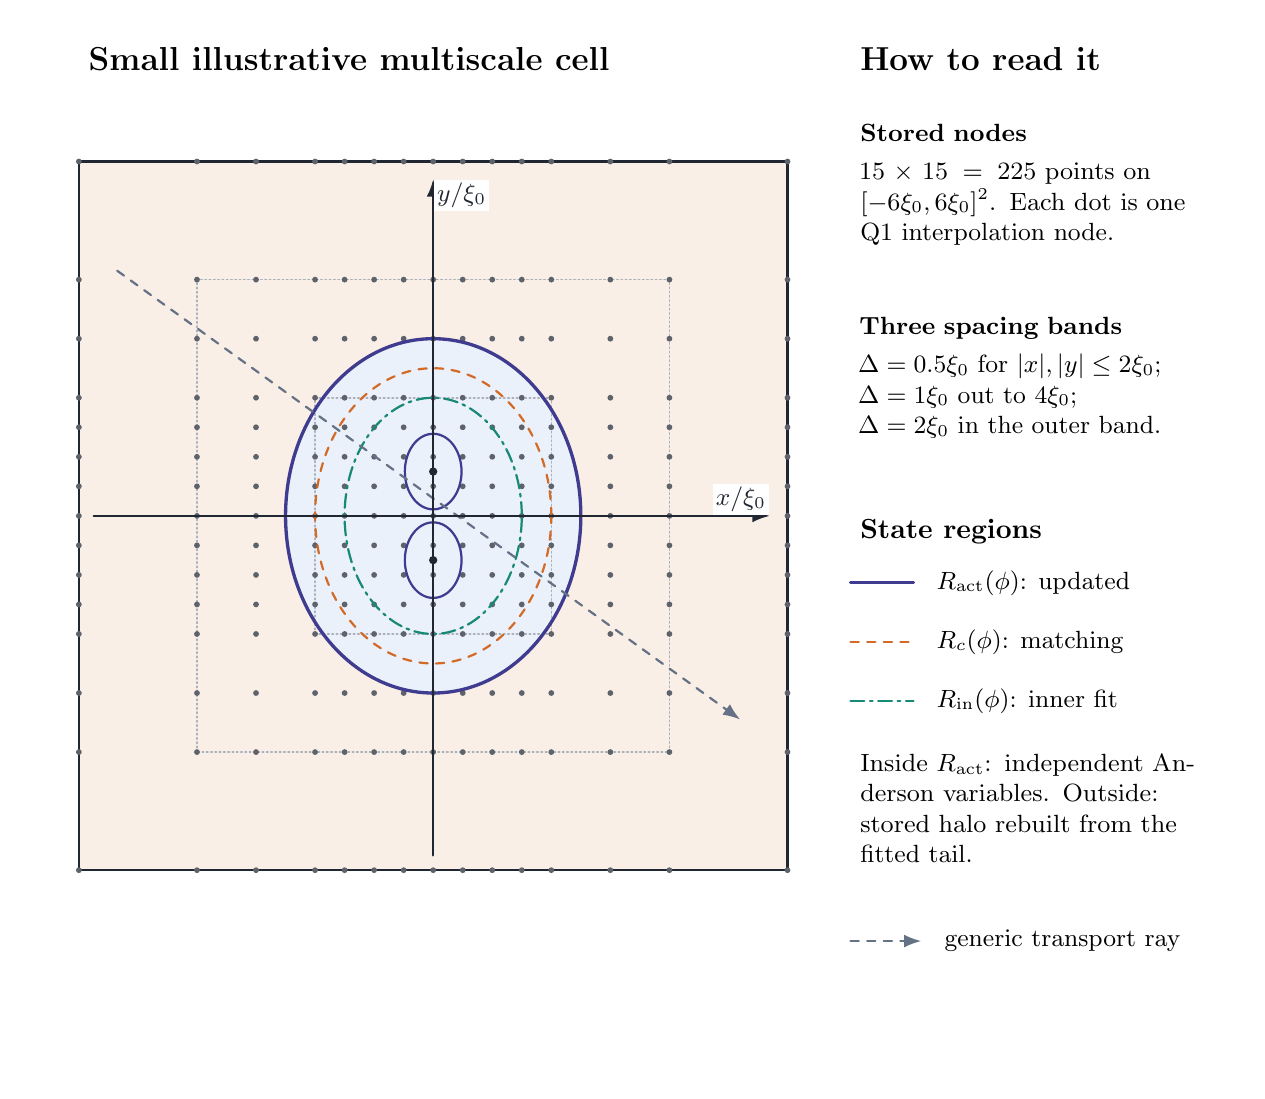
\begin{tikzpicture}[x=1cm,y=1cm,font=\small,line cap=round,line join=round]
  \path[use as bounding box] (0,0) rectangle (15.35,13.25);
  \coordinate (O) at (5.15,7.05);

  \node[anchor=west,font=\large\bfseries] at (0.65,12.85)
    {Small illustrative multiscale cell};
  \node[anchor=west,font=\large\bfseries] at (10.45,12.85)
    {How to read it};

  % Reduced tensor-product mesh: 15 coordinates per direction.
  \def\FFIllustrativeCoordinates{%
    -6,-4,-3,-2,-1.5,-1,-0.5,0,0.5,1,1.5,2,3,4,6}

  % The square [-6,6]^2 is mapped without aspect distortion.
  \begin{scope}[shift={(O)},x=0.75cm,y=0.75cm]
    \clip (-6.12,-6.12) rectangle (6.12,6.12);
    \fill[FFOrangePale] (-6,-6) rectangle (6,6);
    \fill[FFBluePale] (0,0) ellipse [x radius=2.5,y radius=3.0];
    \draw[FFInk,thick] (-6,-6) rectangle (6,6);

    % Boundaries of the fine, medium, and coarse tensor-product zones.
    \draw[FFGray!55,densely dotted,line width=0.55pt]
      (-2,-2) rectangle (2,2);
    \draw[FFGray!55,densely dotted,line width=0.55pt]
      (-4,-4) rectangle (4,4);

    % Every dot is a stored interpolation node in this example cell.
    \foreach \gx in \FFIllustrativeCoordinates {
      \foreach \gy in \FFIllustrativeCoordinates {
        \fill[FFInk!72] (\gx,\gy) circle[radius=1.05pt];
      }
    }

    % Illustrative fit surfaces and independent-update mask.
    \draw[FFIndigo,very thick]
      (0,0) ellipse [x radius=2.5,y radius=3.0];
    \draw[FFOrange,thick,dashed]
      (0,0) ellipse [x radius=2.0,y radius=2.5];
    \draw[FFTeal,thick,dash pattern=on 5pt off 2pt on 1pt off 2pt]
      (0,0) ellipse [x radius=1.5,y radius=2.0];

    % A minimal double-core symbol and one generic quasiclassical trajectory.
    \draw[FFIndigo,thick] (0,0.75) ellipse [x radius=0.48,y radius=0.64];
    \draw[FFIndigo,thick] (0,-0.75) ellipse [x radius=0.48,y radius=0.64];
    \fill[FFInk] (0,0.75) circle[radius=1.5pt];
    \fill[FFInk] (0,-0.75) circle[radius=1.5pt];
    \draw[FFGray,->,thick,dashed] (-5.35,4.15)--(5.20,-3.45);
  \end{scope}

  \begin{scope}[shift={(O)},x=0.75cm,y=0.75cm]
    \draw[->,FFInk,thick] (-5.75,0)--(5.70,0)
      node[above left,fill=white,inner sep=1pt] {$x/\xi_0$};
    \draw[->,FFInk,thick] (0,-5.75)--(0,5.70)
      node[below right,fill=white,inner sep=1pt] {$y/\xi_0$};
  \end{scope}

  % External explanations keep the cell itself uncluttered.
  \node[anchor=north west,align=left,text width=4.35cm] at (10.45,12.15)
    {\textbf{Stored nodes}\\[1mm]
     $15\times15=225$ points on
     $[-6\xi_0,6\xi_0]^2$.  Each dot is one Q1 interpolation node.};

  \node[anchor=north west,align=left,text width=4.35cm] at (10.45,9.70)
    {\textbf{Three spacing bands}\\[1mm]
     $\Delta=0.5\xi_0$ for $|x|,|y|\le2\xi_0$;\\
     $\Delta=1\xi_0$ out to $4\xi_0$;\\
     $\Delta=2\xi_0$ in the outer band.};

  \node[anchor=west,font=\bfseries] at (10.45,6.85) {State regions};
  \draw[FFIndigo,very thick] (10.45,6.20)--(11.25,6.20);
  \node[anchor=west] at (11.42,6.20) {$R_{\rm act}(\phi)$: updated};
  \draw[FFOrange,thick,dashed] (10.45,5.45)--(11.25,5.45);
  \node[anchor=west] at (11.42,5.45) {$R_c(\phi)$: matching};
  \draw[FFTeal,thick,dash pattern=on 5pt off 2pt on 1pt off 2pt]
    (10.45,4.70)--(11.25,4.70);
  \node[anchor=west] at (11.42,4.70) {$R_{\rm in}(\phi)$: inner fit};
  \node[anchor=north west,align=left,text width=4.35cm] at (10.45,4.15)
    {Inside $R_{\rm act}$: independent Anderson variables.  Outside:
     stored halo rebuilt from the fitted tail.};

  \draw[FFGray,->,thick,dashed] (10.45,1.65)--(11.35,1.65);
  \node[anchor=west,align=left,text width=3.75cm] at (11.52,1.65)
    {generic transport ray};
\end{tikzpicture}
\caption{Reduced mesh showing the multiscale-grid principle and the split
between the independent update region and dependent asymptotic halo.  All
$225$ displayed nodes occupy their stated coordinates, but the small cell and
the ellipse sizes are illustrative rather than production-resolution choices.
Line style and direct labels duplicate every colour distinction.}
\label{fig:multiscale-grid-masks}
\end{figure}

\clearpage

\begin{figure}[p]
\centering
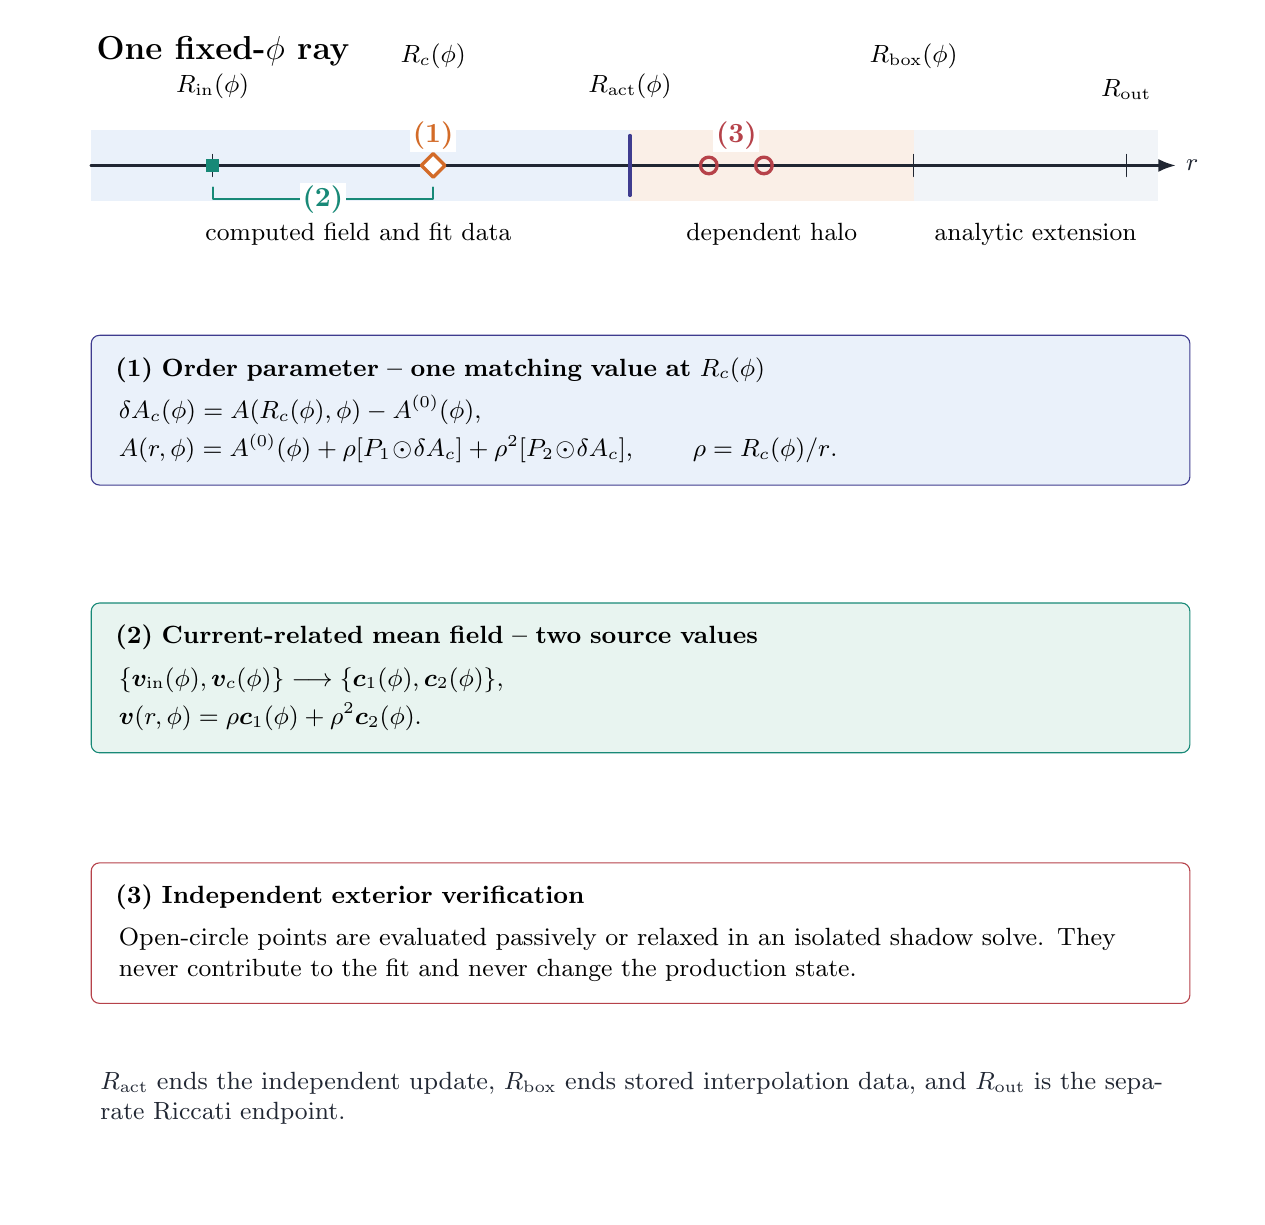
\begin{tikzpicture}[x=1cm,y=1cm,font=\small,line cap=round,line join=round]
  \path[use as bounding box] (0,0) rectangle (15.35,14.85);

  \node[anchor=west,font=\large\bfseries] at (0.75,14.55)
    {One fixed-$\phi$ ray};

  % Radial regions and their five distinct radii.
  \fill[FFBluePale] (0.80,12.65) rectangle (7.65,13.55);
  \fill[FFOrangePale] (7.65,12.65) rectangle (11.25,13.55);
  \fill[FFPale] (11.25,12.65) rectangle (14.35,13.55);
  \draw[->,FFInk,thick] (0.80,13.10)--(14.58,13.10)
    node[right] {$r$};

  \foreach \x in {2.35,5.15,7.65,11.25,13.95}
    \draw[FFInk] (\x,12.96)--(\x,13.24);

  \node[anchor=south] at (2.35,13.82) {$R_{\rm in}(\phi)$};
  \node[anchor=south] at (5.15,14.20) {$R_c(\phi)$};
  \node[anchor=south] at (7.65,13.82) {$R_{\rm act}(\phi)$};
  \node[anchor=south] at (11.25,14.20) {$R_{\rm box}(\phi)$};
  \node[anchor=south] at (13.95,13.82) {$R_{\rm out}$};

  \node[align=center] at (4.20,12.23) {computed field and fit data};
  \node[align=center] at (9.45,12.23) {dependent halo};
  \node[align=center] at (12.80,12.23) {analytic extension};

  % Source markers: shapes and numbers make the colour coding redundant.
  \fill[FFTeal] (2.27,13.02) rectangle (2.43,13.18);
  \draw[FFOrange,very thick,fill=white]
    (5.15,13.10) ++(0,0.15)--++(0.15,-0.15)--++(-0.15,-0.15)--
    ++(-0.15,0.15)--cycle;
  \draw[FFIndigo,very thick] (7.65,12.72)--(7.65,13.48);
  \draw[FFRed,very thick] (8.65,13.10) circle (3.0pt);
  \draw[FFRed,very thick] (9.35,13.10) circle (3.0pt);

  \draw[FFTeal,thick]
    (2.35,12.82)--(2.35,12.67)--(5.15,12.67)--(5.15,12.82);
  \node[FFOrange,font=\bfseries,fill=white,inner sep=1pt] at (5.15,13.48) {(1)};
  \node[FFTeal,font=\bfseries,fill=white,inner sep=1pt] at (3.75,12.67) {(2)};
  \node[FFRed,font=\bfseries,fill=white,inner sep=1pt] at (9.00,13.48) {(3)};

  % Three separated cards replace long routed arrows and crowded labels.
  \node[draw=FFIndigo,rounded corners=3pt,fill=FFBluePale,
        anchor=north west,align=left,text width=13.25cm,
        inner xsep=10pt,inner ysep=8pt] at (0.80,10.95)
    {\textbf{(1) Order parameter -- one matching value at $R_c(\phi)$}\\[1.5mm]
     $\delta A_c(\phi)=A(R_c(\phi),\phi)-A^{(0)}(\phi)$,\\[1mm]
     $A(r,\phi)=A^{(0)}(\phi)
       +\rho[P_1\!\odot\!\delta A_c]
       +\rho^2[P_2\!\odot\!\delta A_c]$,
     \qquad $\rho=R_c(\phi)/r$.};

  \node[draw=FFTeal,rounded corners=3pt,fill=FFGreenPale,
        anchor=north west,align=left,text width=13.25cm,
        inner xsep=10pt,inner ysep=8pt] at (0.80,7.55)
    {\textbf{(2) Current-related mean field -- two source values}\\[1.5mm]
     $\{\bm v_{\rm in}(\phi),\bm v_c(\phi)\}
       \longrightarrow\{\bm c_1(\phi),\bm c_2(\phi)\}$,\\[1mm]
     $\bm v(r,\phi)=\rho\bm c_1(\phi)+\rho^2\bm c_2(\phi)$.};

  \node[draw=FFRed,rounded corners=3pt,fill=white,
        anchor=north west,align=left,text width=13.25cm,
        inner xsep=10pt,inner ysep=8pt] at (0.80,4.25)
    {\textbf{(3) Independent exterior verification}\\[1.5mm]
     Open-circle points are evaluated passively or relaxed in an isolated
     shadow solve.  They never contribute to the fit and never change the
     production state.};

  \node[anchor=west,align=left,text width=13.7cm,FFInk] at (0.80,1.25)
    {$R_{\rm act}$ ends the independent update, $R_{\rm box}$ ends stored
     interpolation data, and $R_{\rm out}$ is the separate Riccati endpoint.};
\end{tikzpicture}
\caption{Asymptotic construction along one fixed-$\phi$ ray.  Numbered
markers identify the order-parameter input, the two mean-field inputs, and
the held-out verification points described in the three cards.  The five
radii have distinct numerical roles; their displayed separations are not to
scale.}
\label{fig:asymptotic-extraction}
\end{figure}

\clearpage

The two-surface construction is the minimum identifiable fit for
\eqref{eq:vasymptotic}.  A later overdetermined annular least-squares fit should
add radial-window and angular-resolution diagnostics without relaxing the
block constraint \eqref{eq:block-tail}.

\section{Nonlinear iteration}

Let $X$ denote the packed real state on the update mask and let
\begin{equation}
  Y=\Fmap(X),\qquad r=Y-X
  \label{eq:fixedpoint}
\end{equation}
be the quasiclassical map and fixed-point residual.  Packing contains the real
and imaginary parts of all nine $A_{\alpha i}$ components followed by the
three real mean-field components.  A masked update preserves every non-update
point exactly before the dependent halo is regenerated.

\subsection{Residual diagnostics}

For $N$ packed values the code reports
\begin{align}
  e_{\rm avg}&=\frac1N\sum_{k=1}^{N}|r_k|,&
  e_{\rm rms}&=\sqrt{\frac1N\sum_{k=1}^{N}r_k^2},\\
  e_{\max}&=\max_k|r_k|,&
  e_{\rm rel}&=\frac{\|r\|_2}{\|X\|_2}.
  \label{eq:residuals}
\end{align}
It also records a legacy scaled maximum and the largest pointwise RMS over 21
values.  Core and outer masks are reported separately so a large quiet region
cannot hide a local defect.  Reaching the iteration limit is a distinct
terminal status and is not renamed convergence.

\subsection{Zero-mode projection}

The double-core solve may remove residual components parallel to numerically
constructed tangents for global gauge, translations, and gauge-compensated
orientation.  A representative orientation tangent is
\begin{equation}
  t_\theta[A]=\ii A+y\,\partial_x A-x\,\partial_y A,
  \label{eq:orientation-tangent}
\end{equation}
with the corresponding spatial rotation of $\bm v$ but no gauge term.  The
tangents are orthogonalised, linearly dependent directions are rejected, and
the removed norm and fraction are reported.  Projection selects a numerical
representative from a symmetry orbit; it does not change the physical
self-consistency equations.

\subsection{Source-compatible Anderson step}

The modern \code{legacy_anderson_t} is a typed transcription of the working
source iterator.  It stores previous iterates $X_i$ and residuals $r_i$,
orders them by residual norm, and finds coefficients $c_i$ that minimise
\begin{equation}
  \left\|r_m+\sum_{i=1}^{m-1}c_i(r_i-r_m)\right\|_2^2.
  \label{eq:anderson-ls}
\end{equation}
Writing
\begin{align}
  d&=\sum_{i=1}^{m-1}c_i(X_i-X_m),\\
  r_{\min}&=r_m+\sum_{i=1}^{m-1}c_i(r_i-r_m),
\end{align}
the accepted candidate is
\begin{equation}
  X_{m+1}=X_m+d+p\,r_{\min},
  \label{eq:anderson-update}
\end{equation}
where the dynamically estimated $p$ is clamped to
$0.01\le p\le p_{\max}$.  The history length grows until its configured limit;
this saturation is expected and does not mean that the residual-minimising
search is disabled.  Poor-progress tests can discard the largest-residual
portion of the retained subspace.  A singular subspace solve invokes the
source-compatible deterministic sinusoidal fallback and is reported.

In the nonsingular branch the source-compatible mixing estimate is
\begin{equation}
  \eta=\min\!\left(1,
    \sqrt{\frac{R_{\min}^{\rm previous}}{\|r_{\rm current}\|_2^2}}\right),
  \qquad
  p=\operatorname{clip}_{[0.01,p_{\max}]}
  \left\{\frac{\eta}{2}
  \left(\frac{\|d\|_2}{\|r_{\rm base}\|_2}+p_{\rm old}\right)\right\}.
  \label{eq:anderson-p}
\end{equation}
The first update is the simple step $X_{1}=X_0+0.01r_0$.  The implemented
stopping rule is the unnormalised condition $\max_k|r_k|\le\varepsilon$; the
other residual measures remain essential diagnostics.

Only rank zero owns the Anderson history and performs this update.  The next
typed field and its reports are broadcast to all ranks.  Checkpoints contain
the field, not the Anderson history; a restart therefore begins a fresh
accelerator history.

\section{End-to-end algorithm}

Figure~\ref{fig:algorithm-flow} shows the current production path.  The outer
loop is a fixed-mesh solve.  Post-solve exterior validation is intentionally
outside that loop and cannot modify the accepted production state.

\begin{landscape}
\begin{figure}[p]
\centering
\resizebox{\linewidth}{!}{%
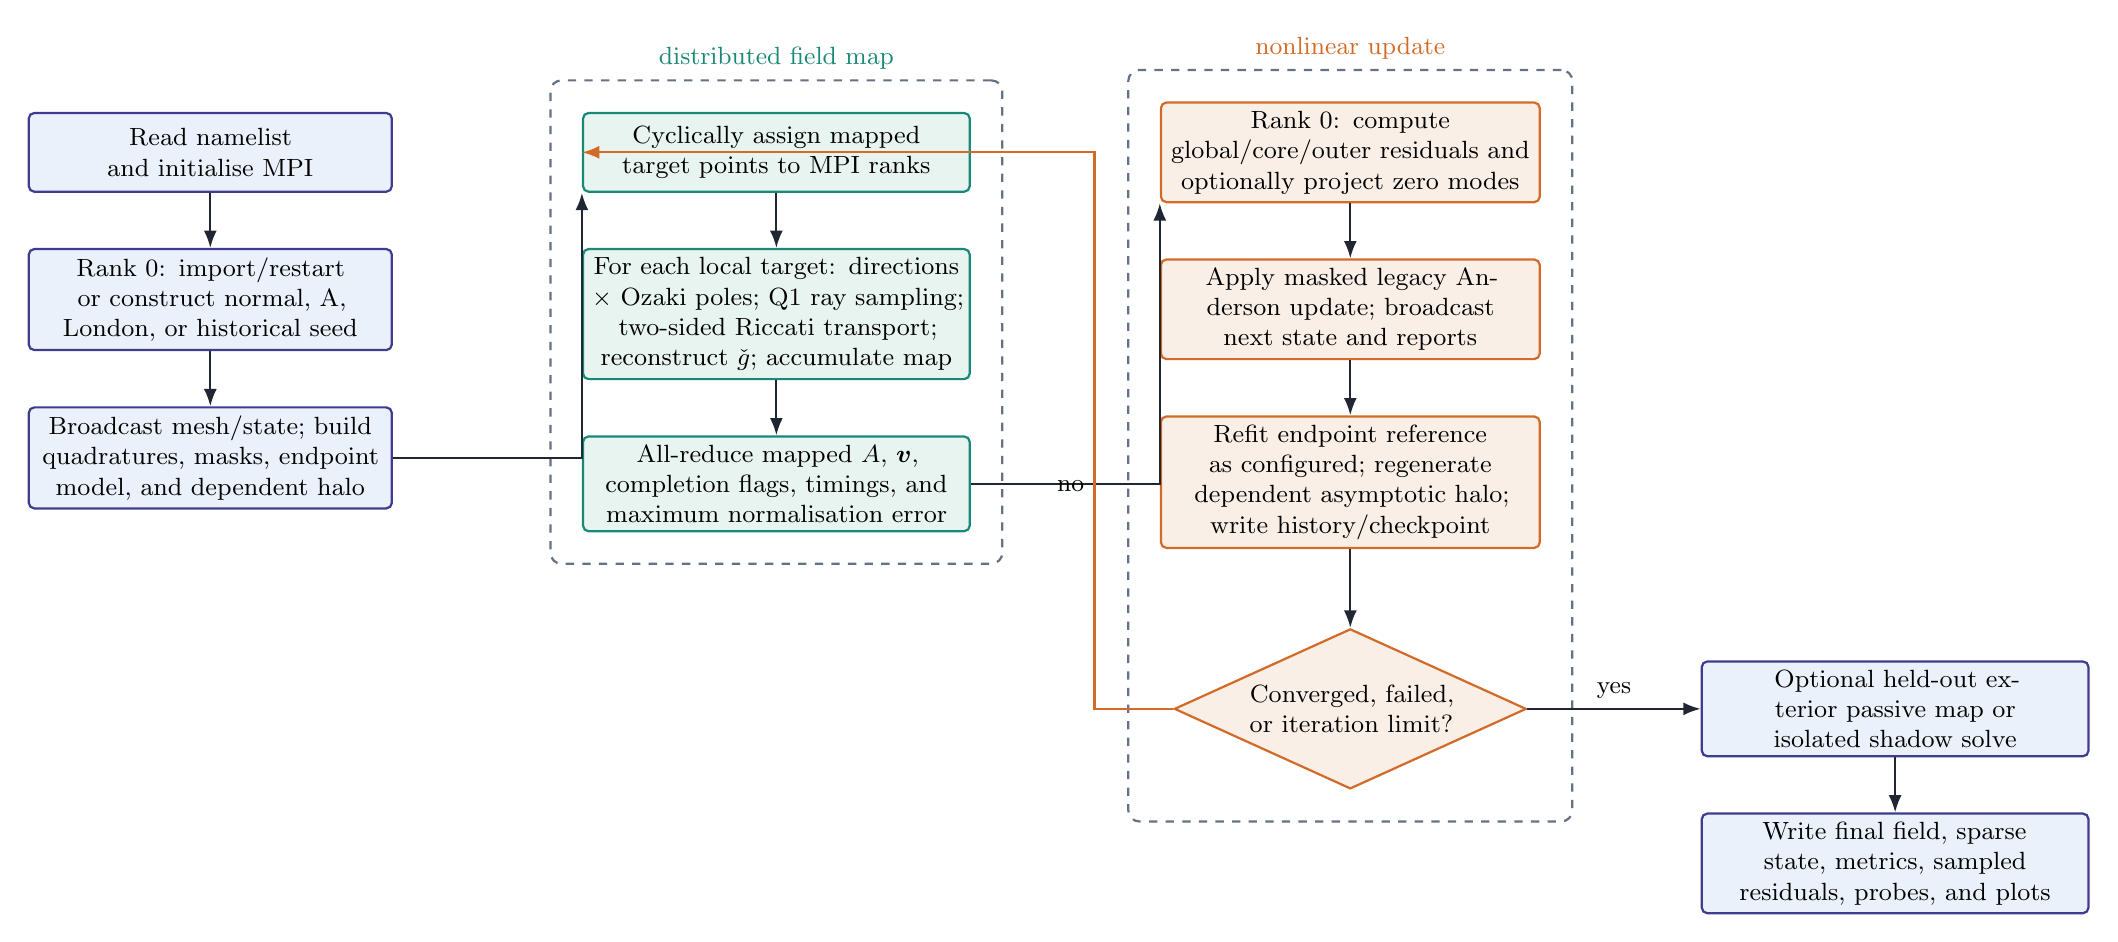
\begin{tikzpicture}[node distance=7mm and 13mm, font=\small]
  \node[ffbox, text width=44mm] (input) {Read namelist and initialise MPI};
  \node[ffbox, below=of input, text width=44mm] (init)
    {Rank 0: import/restart or construct normal, A, London, or historical seed};
  \node[ffbox, below=of init, text width=44mm] (setup)
    {Broadcast mesh/state; build quadratures, masks, endpoint model, and dependent halo};

  \node[ffgreen, right=24mm of input, text width=47mm] (distribute)
    {Cyclically assign mapped target points to MPI ranks};
  \node[ffgreen, below=of distribute, text width=47mm] (pointmap)
    {For each local target: directions $\times$ Ozaki poles; Q1 ray sampling; two-sided Riccati transport; reconstruct $\check g$; accumulate map};
  \node[ffgreen, below=of pointmap, text width=47mm] (reduce)
    {All-reduce mapped $A$, $\bm v$, completion flags, timings, and maximum normalisation error};

  \node[fforange, right=24mm of distribute, text width=46mm] (residual)
    {Rank 0: compute global/core/outer residuals and optionally project zero modes};
  \node[fforange, below=of residual, text width=46mm] (anderson)
    {Apply masked legacy Anderson update; broadcast next state and reports};
  \node[fforange, below=of anderson, text width=46mm] (halo)
    {Refit endpoint reference as configured; regenerate dependent asymptotic halo; write history/checkpoint};
  \node[ffdecision, below=10mm of halo] (stop) {Converged, failed, or iteration limit?};

  \node[ffbox, right=22mm of stop, text width=47mm] (shadow)
    {Optional held-out exterior passive map or isolated shadow solve};
  \node[ffbox, below=of shadow, text width=47mm] (output)
    {Write final field, sparse state, metrics, sampled residuals, probes, and plots};

  \draw[ffarrow] (input)--(init);
  \draw[ffarrow] (init)--(setup);
  \draw[ffarrow] (setup.east)-| (distribute.south west);
  \draw[ffarrow] (distribute)--(pointmap);
  \draw[ffarrow] (pointmap)--(reduce);
  \draw[ffarrow] (reduce.east)-| (residual.south west);
  \draw[ffarrow] (residual)--(anderson);
  \draw[ffarrow] (anderson)--(halo);
  \draw[ffarrow] (halo)--(stop);
  \draw[ffreturn] (stop.west) -- ++(-10mm,0) |- node[pos=0.20,left]{no} (distribute.west);
  \draw[ffarrow] (stop.east) -- node[above]{yes} (shadow.west);
  \draw[ffarrow] (shadow)--(output);

  \begin{scope}[on background layer]
    \node[ffgroup, fit=(distribute)(pointmap)(reduce),
      label={[text=FFTeal]above:distributed field map}] {};
    \node[ffgroup, fit=(residual)(anderson)(halo)(stop),
      label={[text=FFOrange]above:nonlinear update}] {};
  \end{scope}
\end{tikzpicture}
}
\caption{Implemented production algorithm.  The expensive bracket is repeated
for every nonlinear update.  The independent exterior check is a validation
stage and never feeds back into the production solution.}
\label{fig:algorithm-flow}
\end{figure}
\end{landscape}

\subsection{One mapped target point}

For one target node $a$, the map can be expressed as the following nested
algorithm:
\begin{enumerate}
  \item For each angular quadrature direction, intersect the projected ray
  with the rectangular mesh, insert $s=0$, limit path spacing, and cache Q1
  stencils.
  \item Sample $A$ and $\bm v$ on the interior path.  If the free-vortex
  endpoint is enabled, extend the path through the analytic exterior to its
  enclosing circle.
  \item For each positive Ozaki pole, integrate the entry-stable and
  exit-stable coherence branches to the target using \eqref{eq:riccati0}--
  \eqref{eq:substeps}.
  \item Convert both source coefficient sets to spin matrices and reconstruct
  $\check g$ using \eqref{eq:reconstruction}.  Reject singular reconstruction;
  otherwise update \eqref{eq:normerror}.
  \item Accumulate \eqref{eq:gapmap}--\eqref{eq:currentmap}; after all
  directions and poles, apply $C_\Delta$ to the gap part only.
\end{enumerate}

The natural unit of parallel work is therefore a target--direction--pole ray.
The current CPU/MPI implementation distributes only target points, while the
direction--pole loops remain available for later threaded or GPU batching.

\section{Current code construction}

The CMake build separates reusable non-MPI physics/data code in the
\code{he3_mesh} library from MPI execution code in
\code{he3_mpi_execution}.  The double-core application source is exposed both
under its benchmark name and as the user-facing
\code{fermiforge_double_core_2d} executable.  Figure~\ref{fig:module-flow}
shows the principal call direction, not every Fortran \code{use} association.

\begin{landscape}
\begin{figure}[p]
\centering
\resizebox{0.88\linewidth}{!}{%
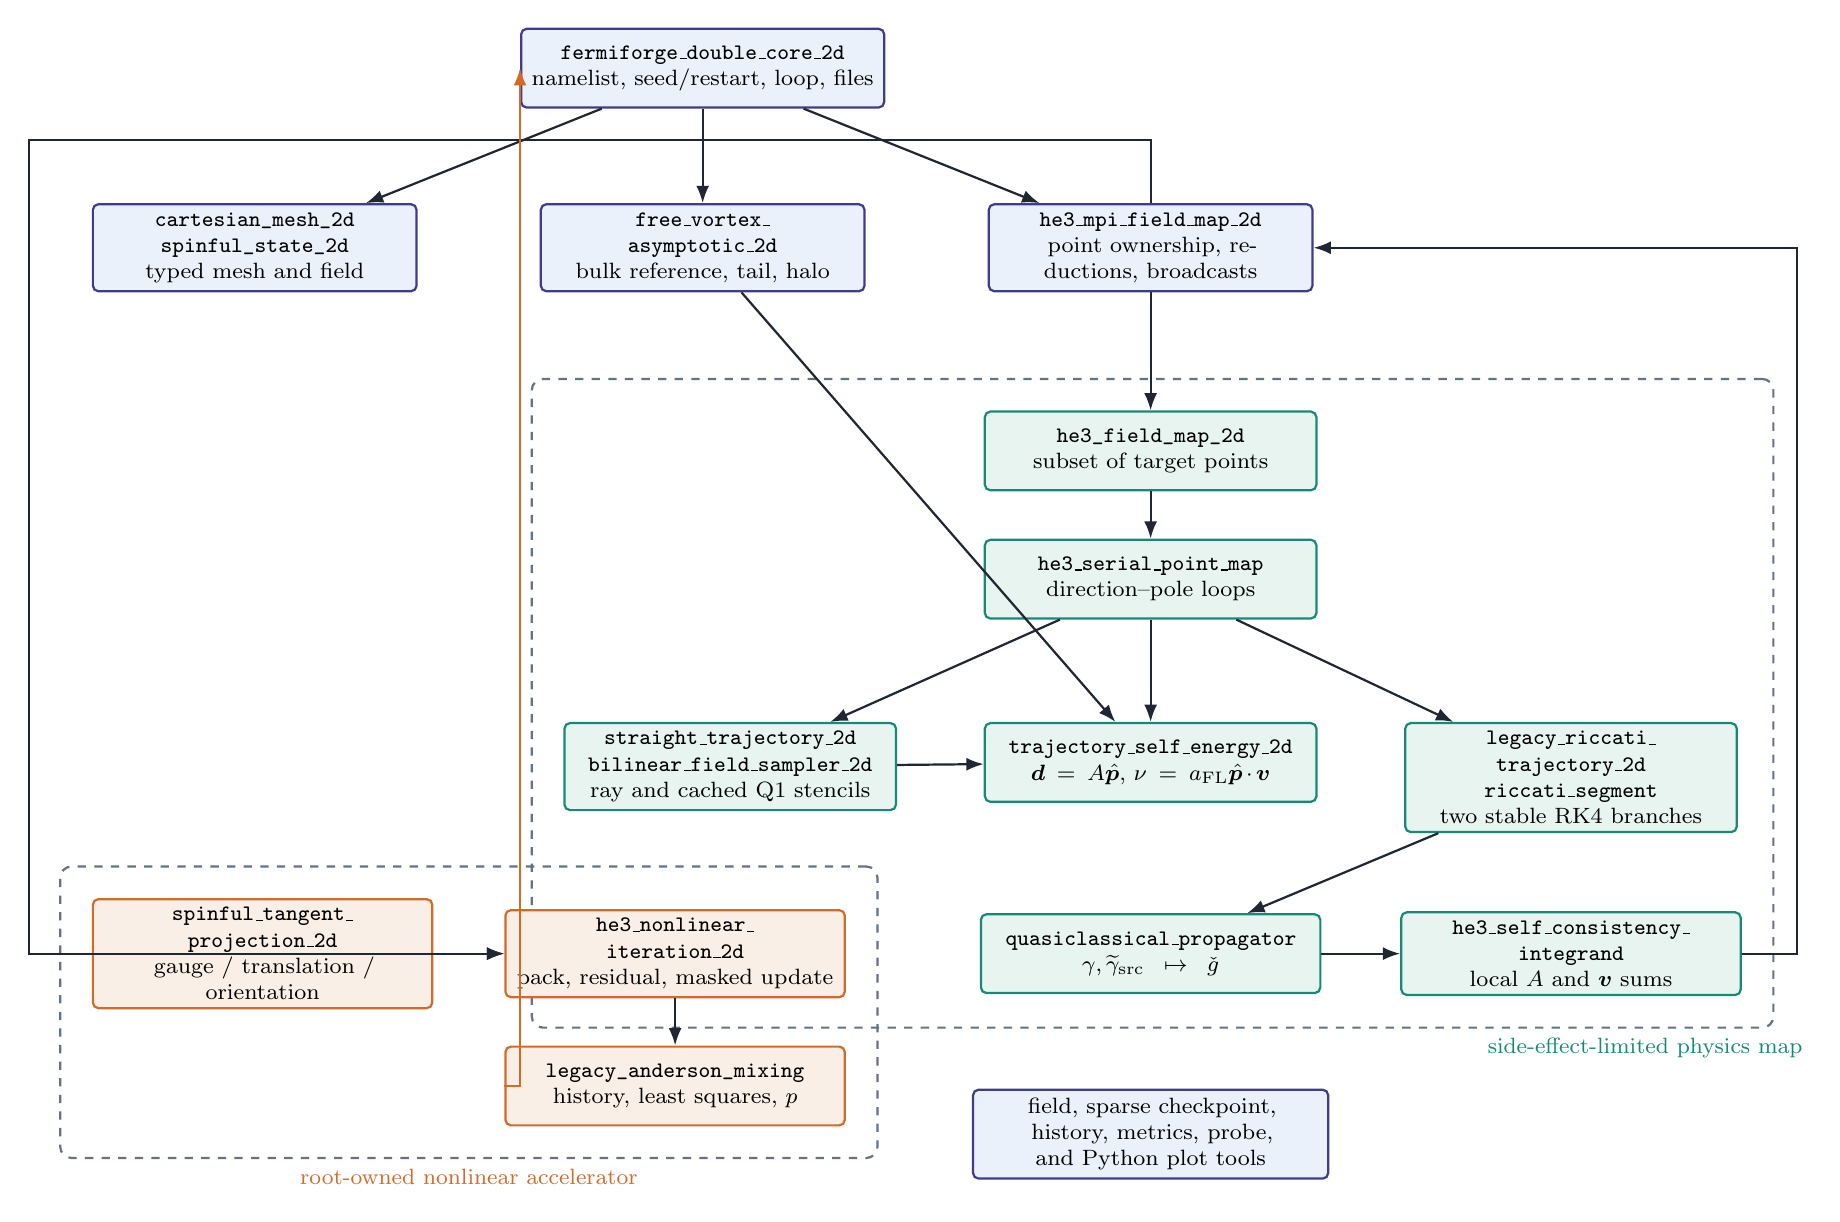
\begin{tikzpicture}[node distance=6mm and 8mm, font=\footnotesize]
  \node[ffbox, text width=44mm] (app)
    {\texttt{fermiforge\_double\_core\_2d}\\namelist, seed/restart, loop, files};

  \node[ffbox, below left=12mm and 13mm of app, text width=39mm] (data)
    {\code{cartesian_mesh_2d}\\\code{spinful_state_2d}\\typed mesh and field};
  \node[ffbox, below=12mm of app, text width=39mm] (endpoint)
    {\texttt{free\_vortex\_}\\\texttt{asymptotic\_2d}\\bulk reference, tail, halo};
  \node[ffbox, below right=12mm and 13mm of app, text width=39mm] (mpi)
    {\texttt{he3\_mpi\_field\_map\_2d}\\point ownership, reductions, broadcasts};

  \node[ffgreen, below=15mm of mpi, text width=40mm] (field)
    {\code{he3_field_map_2d}\\subset of target points};
  \node[ffgreen, below=of field, text width=40mm] (serial)
    {\texttt{he3\_serial\_point\_map}\\direction--pole loops};

  \node[ffgreen, below left=13mm and 11mm of serial, text width=40mm] (ray)
    {\texttt{straight\_trajectory\_2d}\\\texttt{bilinear\_field\_sampler\_2d}\\ray and cached Q1 stencils};
  \node[ffgreen, below=13mm of serial, text width=40mm] (se)
    {\texttt{trajectory\_self\_energy\_2d}\\$\bm d=A\phat$, $\nu=a_{\rm FL}\phat\!\cdot\!\bm v$};
  \node[ffgreen, below right=13mm and 11mm of serial, text width=40mm] (riccati)
    {\texttt{legacy\_riccati\_}\\\texttt{trajectory\_2d}\\\texttt{riccati\_segment}\\two stable RK4 branches};

  \node[ffgreen, below=14mm of se, text width=41mm] (prop)
    {\texttt{quasiclassical\_propagator}\\
     $\gamma,\widetilde\gamma_{\rm src}\mapsto\check g$};
  \node[ffgreen, right=10mm of prop, text width=41mm] (sc)
    {\texttt{he3\_self\_consistency\_}\\\texttt{integrand}\\local $A$ and $\bm v$ sums};

  \node[fforange, left=17mm of prop, text width=41mm] (nonlinear)
    {\texttt{he3\_nonlinear\_}\\\texttt{iteration\_2d}\\pack, residual, masked update};
  \node[fforange, below=of nonlinear, text width=41mm] (aa)
    {\code{legacy_anderson_mixing}\\history, least squares, $p$};
  \node[fforange, left=9mm of nonlinear, text width=41mm] (zero)
    {\texttt{spinful\_tangent\_}\\\texttt{projection\_2d}\\gauge / translation /\\orientation};

  \node[ffbox, below=12mm of prop, text width=43mm] (io)
    {field, sparse checkpoint, history, metrics, probe, and Python plot tools};

  \draw[ffarrow] (app)--(data);
  \draw[ffarrow] (app)--(endpoint);
  \draw[ffarrow] (app)--(mpi);
  \draw[ffarrow] (mpi)--(field);
  \draw[ffarrow] (field)--(serial);
  \draw[ffarrow] (serial)--(ray);
  \draw[ffarrow] (serial)--(se);
  \draw[ffarrow] (serial)--(riccati);
  \draw[ffarrow] (ray)--(se);
  \draw[ffarrow] (endpoint)--(se);
  \draw[ffarrow] (riccati)--(prop);
  \draw[ffarrow] (prop)--(sc);
  \draw[ffarrow] (sc.east) -- ++(7mm,0) |- (mpi.east);
  \draw[ffarrow] (mpi.north) -- ++(0,8mm)
    -| ($(data.west)+(-8mm,0)$) |- (nonlinear.west);
  \draw[ffarrow] (zero)--(nonlinear);
  \draw[ffarrow] (nonlinear)--(aa);
  \draw[ffreturn] (aa.west) -| (app.west);

  \begin{scope}[on background layer]
    \node[ffgroup, fit=(field)(serial)(ray)(se)(riccati)(prop)(sc),
      label={[text=FFTeal]below right:side-effect-limited physics map}] {};
    \node[ffgroup, fit=(zero)(nonlinear)(aa),
      label={[text=FFOrange]below:root-owned nonlinear accelerator}] {};
  \end{scope}
\end{tikzpicture}
}
\caption{Principal implemented module pipeline.  The reusable physics path is
kept separate from MPI orchestration and from the application-level workflow.}
\label{fig:module-flow}
\end{figure}
\end{landscape}

\subsection{MPI execution model}

If active points are numbered $a=0,\ldots,N_a-1$, rank $r$ of $P$ receives
points satisfying $a\bmod P=r$.  Each rank maps its local targets into a
zero-initialised full-size output.  \code{MPI_Allreduce} with a sum then
assembles the unique active contributions; inactive points are copied exactly
from the input state.  Counts and timing sums are reduced, while the maximum
normalisation error and rank elapsed time use a maximum reduction.

This replicated-state design is simple and already verifies equal numerical
answers at multiple rank counts.  It is not a spatial domain decomposition:
there are no mesh-halo exchanges, and memory per rank grows with the full
field.  The first GPU stage can retain this model, batching direction--pole
rays within each rank; larger meshes will eventually require a measured choice
between distributed spatial blocks and direction/energy decomposition.

\subsection{Checkpoint and output semantics}

Dense field files contain coordinates, 18 real order-parameter entries, a
pair-density proxy, and the three current-related mean-field components.
Sparse checkpoints contain coordinates plus the 21 nonlinear values at a
selected checkpoint mask.  Restart overlays values onto exact mesh nodes and
starts a new Anderson history.

Post-processing can transform the Cartesian $3\times3$ field to the frozen
complex cylindrical/harmonic basis used by the radial source.  These harmonic
components are diagnostics and plotting products; the unconstrained 2D solver
continues to store and interpolate the Cartesian tensor directly.

On an iteration-limited run, the final field/checkpoint contains the last
\emph{accepted} state, while the production residual describes the last
evaluated pair $X\mapsto\Fmap(X)$ before that acceptance.  This distinction
should be retained when comparing a plotted state with the last residual line.

\section{Exterior verification and acceptance diagnostics}

The asymptotic formula is part of the production boundary model, so evaluating
it at the same points used to determine its coefficients is not an independent
test.  The implemented validation layer therefore adds exterior mesh points
that are not production unknowns.

Let $B$ be the frozen final production state on all ordinary points and let
$P$ denote a small mask of held-out exterior points.  Two modes are available:
\begin{description}[leftmargin=31mm,style=nextline]
  \item[Passive defect] Evaluate $\Fmap(B)-B$ on $P$.  This tests whether the
  extrapolated value is locally consistent with the microscopic map without
  changing it.
  \item[Shadow iteration] Keep every point outside $P$ fixed, initialise an
  independent Anderson accelerator, and relax only $P$ to a state $S^*$.  The
  output stores $B$, the first map $\Fmap(B)$, $S^*$, and the terminal map
  $\Fmap(S^*)$.
\end{description}
The useful quantities are
\begin{align}
  \delta_{\rm passive}&=\Fmap(B)-B,\\
  \delta_{\rm correction}&=S^*-B,\\
  \delta_{\rm terminal}&=\Fmap(S^*)-S^*.
  \label{eq:shadow}
\end{align}
The correction is interpretable as an independently relaxed discrepancy only
when the shadow solve reaches its stated convergence tolerance.  A
\code{shadow_not_converged} result is diagnostic data, not a converged
correction.  The shadow state, history, and maps never alter production
checkpoints, endpoint fits, or convergence status.

The minimum acceptance set for a physical double-core solution should include:
\begin{itemize}
  \item nonlinear residuals resolved by hard-core, soft-core, and exterior
  zones;
  \item $\epsilon_{\rm norm}$ from \eqref{eq:normerror};
  \item mesh, active-domain, matching-surface, outer-circle, trajectory-step,
  direction, and Ozaki-pole convergence studies;
  \item stability of the half-core separation and relevant harmonics;
  \item passive and, when affordable, converged shadow exterior defects;
  \item agreement with radial normal- and A-core references in the symmetric
  limit and with archived double-core data when imported;
  \item symmetry checks and, before claiming energetic stability, a consistent
  free-energy comparison.
\end{itemize}

\section{Observable and terminology safeguards}

The plotted pair-density proxy is
\begin{equation}
  n_{\rm pair}^{\rm proxy}(\bm r)=
  \frac13\sum_{\alpha i}|A_{\alpha i}(\bm r)|^2.
  \label{eq:pairdensity}
\end{equation}
It is useful for locating half cores but is not the response-defined
superfluid density.  Likewise, $\bm v$ and \eqref{eq:currentmap} are
current-related Fermi-liquid fields rather than a normalised physical mass
current.  A future observable layer must freeze energy and length units, field
normalisation, and all physical prefactors before labels such as
$\rho_s$ or SI current density are used.

The implementation has the full complex triplet tensor and spin-matrix
propagator, but ``full spin'' currently has defined limits: the diagonal
spin-exchange self-energy is zero, singlet/mixed pairing is absent, and no
spin-active interface boundary condition is connected.  Those are extensions
of the field/self-energy model, not merely larger arrays.

The historical arrays also do not by their type prove whether the stored
code-basis tensor is exactly the manuscript's $A$ or its constant-rotation and
bulk-amplitude-reduced $\widetilde A$.  Until that conversion and the code
length/energy units are frozen by a documented regression, this note keeps the
neutral name ``code-basis $A$'' and avoids attaching an unverified unit symbol
to every plotted coordinate.

\section{Verification ladder}

Development follows a ladder in which each new layer retains a lower-level
oracle:
\begin{enumerate}
  \item manufactured constant, affine, and bilinear fields test mesh lookup
  and Q1 interpolation;
  \item radial harmonic conversion and Cartesian embedding test basis and
  phase conventions;
  \item frozen trajectory checkpoints test the two legacy Riccati branches;
  \item arbitrary nonsingular coherence matrices test reconstruction and
  \eqref{eq:normerror};
  \item a complete one-point map tests direction/pole accumulation;
  \item radial versus 2D point maps test the spatial bridge;
  \item one-, four-, and ten-rank runs test MPI invariance;
  \item normal-core 2D relaxation tests the nonlinear loop;
  \item A-phase-core runs stress the long $1/r$ soft tail;
  \item double-core runs test broken axial symmetry, moving half cores,
  angle-dependent asymptotics, and zero modes;
  \item held-out exterior probes test the asymptotic closure independently.
\end{enumerate}

The seed family is also provenance-labelled.  Radial normal/A solutions are
reference embeddings; \code{nop}, \code{aop}, and \code{dop} reproduce the
historical initialisation logic; the regularised London double-core seed is a
smooth model seed, not the same object as historical \code{dop}; imported
legacy 2D fields provide a later numerical oracle.

\section{What is not yet implemented}

\begin{tabularx}{\textwidth}{>{\raggedright\arraybackslash}p{34mm}X}
\toprule
Topic & Present boundary of the implementation\\
\midrule
Spatial adaptation & Fine/medium/coarse tensor-product mesh and staged active
ellipse changes exist.  There is no quadtree, local error-driven refinement,
two-to-one balancing, or automatic field transfer/restart.\\
Walls and devices & The general 2D solver has a free-vortex analytic exterior.
Specular reflection exists only in historical work and is not connected to
the modern 2D transport path.  Leads, weak links, diffuse scattering, and
spin-active interfaces are future work.\\
Long-scale physics & The asymptotic spin-rotation tail is represented, but a
self-consistent dipole term and a multilevel texture solver are not connected.\\
Accelerators & Kernels and data flow are being separated for batching, but no
OpenMP-target, OpenACC, CUDA, HIP, or SYCL offload path is implemented.\\
DG/FEM & The discontinuous-Galerkin approach of Seja and
Löfwander~\cite{seja2022} is a target architecture for general devices, not a
feature of the present Q1-sampled ray solver.  DG is a finite-element method,
not a finite-difference method.\\
Scaling & MPI distributes target points with a replicated field.  Functional
rank agreement has been tested; production strong/weak scaling and
multi-node memory limits have not yet been established.\\
Thermodynamics & A fully normalised physical current, superfluid-density
tensor, free-energy functional, and stability comparison are not yet part of
the modern output layer.\\
\bottomrule
\end{tabularx}

\section{Development path from this architecture}

The logical sequence is governed by verification gates rather than by replacing
all infrastructure at once.

\begin{enumerate}
  \item \textbf{Accept the free-vortex 2D reference.}  Obtain reproducible
  normal-, A-, and double-core solutions; quantify domain, tail, quadrature,
  transport, and nonlinear convergence; compare against radial and archived
  2D data.
  \item \textbf{Turn staged multiscale studies into block adaptation.}  Add
  dense rectangular blocks, conservative restriction/prolongation, local
  residual and gradient indicators, two-to-one balance, and solve--estimate--
  transfer--restart cycles.  Rebuild ray stencils and reset Anderson whenever
  the mesh changes.
  \item \textbf{Add a geometry and scattering interface.}  Geometry supplies
  inside/outside tests, intersections, normals, and material identifiers;
  scattering supplies specular, diffuse, partially specular, or spin-active
  laws.  For a specular wall with normal $\hat{\bm n}$,
  \begin{equation}
    \phat_{\rm out}=\phat_{\rm in}
      -2(\phat_{\rm in}\cdot\hat{\bm n})\hat{\bm n},
  \end{equation}
  while $p_z$ is conserved for a wall extruded along the invariant axis.
  \item \textbf{Evaluate the DG transition.}  Use the validated point-map
  physics as an oracle while introducing the discontinuous-Galerkin weak form
  for general geometries.  Decide polynomial order, flux/boundary treatment,
  and adaptivity from measured accuracy and cost rather than terminology.
  \item \textbf{Batch the ray kernel and offload portably.}  First build a
  structure-of-arrays batched CPU path.  Then use a thin OpenMP-target
  execution layer as the initial vendor-neutral route, retaining identical
  physics kernels and a CPU reference.  MPI remains the multi-node layer.
  \item \textbf{Generalise material self-energies and observables.}  Add
  singlet/triplet mixtures, exchange fields, impurity/interface terms, physical
  current/free energy, walls, weak links, and superconducting--magnetic
  devices behind explicit model interfaces.
\end{enumerate}

This ordering preserves a trusted reference at each step: radial source
$\rightarrow$ modern scalar CPU map $\rightarrow$ 2D MPI relaxation
$\rightarrow$ adaptive/DG CPU solver $\rightarrow$ batched accelerator solver.

\section{Reproducibility checklist for a run}

A result should archive enough information to reconstruct both the physical
map and the numerical approximation:
\begin{itemize}
  \item Git revision and statement of any uncommitted changes;
  \item compiler, build type, MPI implementation, and rank count;
  \item complete namelist plus the exact Gauss and Ozaki tables;
  \item seed type or restart path and the bulk-reference policy;
  \item explicit $x$ and $y$ coordinates, update/mapped/checkpoint masks, and
  all circular/elliptical fit radii;
  \item trajectory step, Riccati substep floor, endpoint relaxation distance,
  outer circle, and asymptotic policy;
  \item Anderson history limit, $p_{\max}$, projection policy, tolerance, and
  terminal status;
  \item iteration history, final accepted state, last evaluated residual,
  propagator-normalisation maximum, and shadow status;
  \item plotting scripts and colour-scale conventions used for the figures.
\end{itemize}

\appendix
\section{Compact pseudocode}

\begin{verbatim}
MPI initialise
rank 0: read input; import/restart or construct seed
broadcast mesh and full state
read angular and Ozaki rules; configure endpoint and masks
regenerate dependent asymptotic halo

for nonlinear iteration:
    distribute mapped target points cyclically over ranks
    for each local target point:
        accumulator = 0
        for each angular direction:
            build projected ray and cached Q1 stencils
            sample A and current-related field
            extend ray through analytic exterior when enabled
            for each positive Ozaki pole:
                integrate stable coherence from entry to target
                integrate stable reverse branch from exit to target
                reconstruct 4x4 propagator; check g^2 = -1
                accumulate gap and mean-field contributions
        finalise target map
    all-reduce mapped state and diagnostics
    rank 0: compute residuals; optionally remove zero modes
    rank 0: Anderson update on update mask
    broadcast accepted state
    refit configured bulk reference; regenerate dependent halo
    write history/checkpoint; test stop condition

optional: freeze production state and evaluate/iterate held-out exterior probes
rank 0: write final fields, metrics, residuals, probes, plots
MPI finalise
\end{verbatim}

\section{Principal source-to-module correspondence}

\begin{longtable}{>{\raggedright\arraybackslash}p{43mm}p{94mm}}
\toprule
Concern & Current module or application layer\\
\midrule
\endfirsthead
\toprule
Concern & Current module or application layer\\
\midrule
\endhead
Typed mesh and state & \code{cartesian_mesh_2d}, \code{spinful_state_2d}\\
Iteration packing & \code{new_src_iteration_layout_2d}\\
Q1 interpolation and rays & \code{bilinear_field_sampler_2d},
\code{straight_trajectory_2d}\\
Trajectory self-energy & \code{trajectory_self_energy_2d}\\
Riccati propagation & \code{riccati_segment},
\code{legacy_riccati_trajectory_2d}\\
Spin--Nambu reconstruction & \code{spin_matrix_2x2},
\code{quasiclassical_propagator}\\
Quadrature and point map & \code{he3_quadrature},
\code{he3_self_consistency_integrand}, \code{he3_serial_point_map}\\
Field and MPI maps & \code{he3_field_map_2d},
\code{he3_mpi_field_map_2d}\\
Asymptotic exterior & \code{free_vortex_asymptotic_2d}\\
Residual and Anderson update & \code{he3_nonlinear_iteration_2d},
\code{legacy_anderson_mixing}\\
Zero modes & \code{spinful_tangent_projection_2d}\\
Seeds & \code{double_core_seed_2d}, \code{historical_core_seed_2d}, radial
embedding/import modules\\
Application workflow & \code{app/benchmark_legacy_double_core_map_2d.f90},
built as \code{fermiforge_double_core_2d}\\
Run orchestration and plots & scripts in \code{tools/}\\
\bottomrule
\end{longtable}

\begin{thebibliography}{9}

\bibitem{dcvlong}
M.~A. Silaev, E.~V. Thuneberg, and M. Fogelstr\"om,
``Structure, bound states, and rotational dynamics of the double-core vortex
in superfluid $^3$He-B,'' working manuscript, 11 September 2026.  In
particular, Eqs.~(1), (19), and (20) supply the order-parameter and asymptotic
conventions used here.

\bibitem{serene1983}
J.~W. Serene and D. Rainer,
``The quasiclassical approach to superfluid $^3$He,''
\emph{Physics Reports} \textbf{101}, 221--311 (1983),
\href{https://doi.org/10.1016/0370-1573(83)90051-0}
{doi:10.1016/0370-1573(83)90051-0}.

\bibitem{eschrig2000}
M. Eschrig,
``Distribution functions in nonequilibrium theory of superconductivity and
Andreev spectroscopy in unconventional superconductors,''
\emph{Phys. Rev. B} \textbf{61}, 9061 (2000),
\href{https://doi.org/10.1103/PhysRevB.61.9061}
{doi:10.1103/PhysRevB.61.9061}.

\bibitem{ozaki2007}
T. Ozaki,
``Continued fraction representation of the Fermi--Dirac function for
large-scale electronic structure calculations,''
\emph{Phys. Rev. B} \textbf{75}, 035123 (2007),
\href{https://doi.org/10.1103/PhysRevB.75.035123}
{doi:10.1103/PhysRevB.75.035123}.

\bibitem{seja2022}
K.~M. Seja and T. L\"ofwander,
``Finite element method for the quasiclassical theory of superconductivity,''
\emph{Phys. Rev. B} \textbf{106}, 144511 (2022),
\href{https://doi.org/10.1103/PhysRevB.106.144511}
{doi:10.1103/PhysRevB.106.144511}.

\end{thebibliography}

\end{document}
